\chapter{Teoria degli insiemi}
\section{Definizione e rappresentazione degli insiemi}
Il concetto di insieme è un concetto primitivo, ovvero non è possibile definirlo in termini di altri concetti. Un insieme è una collezione di oggetti, detti elementi, che possono essere di qualsiasi tipo. Agli albori della teoria degli insiemi si pensava che ogni insieme fosse l'\textbf{estensione di un predicato}, ovvero l'insieme di tutti gli oggetti che soddisfano una determinata proprietà.

\dfn{Estensione di un predicato}{\index{Predicato!Estensione di}
	Sia $\varphi = \varphi(x)$ un predicato unario nella variabile $x$. Si indica col simbolo $E_{\varphi}=\{x \; | \; \varphi \}$ la totalità degli oggetti $a$ che, sostituiti ad $x$ in $\varphi$, rendono $\varphi$ vera ($\varphi(a)$ è una formula vera). Questa totalità prende il nome di \textbf{estensione} di $\varphi$ che può essere anche scritta mediante la formula:
	\begin{equation}
		\forall x (x \in E_{\varphi} \iff \varphi(x))
	\end{equation}
}

Il tentativo di fondare l'intera teoria sull'idea che l'estensione di ogni predicato unario si potesse considerare come insieme fallì non appena si scoprì che questa assunzione portava necessariamente a delle contraddizioni. Non sempre infatti l'estensione $\{x \; | \; \varphi \}$ di un predicato $\varphi$ è un insieme\footnote{Esistono proprietà perfettamente ragionevoli e ben definite tali che non esista l'insieme degli oggetti che le verificano.} come dimostrò Bertrand Russell\index{Bertrand Russell} mediante il suo omonimo paradosso. Limitando però la ricerca degli oggetti ai soli elementi di un insieme $s$ allora sicuramente è possibile considerare l'insieme degli elementi di $s$ che verificano quella data proprietà $\varphi$.  Questo è assicurato da uno degli assiomi della teoria degli insiemi, ovvero l'\textbf{assioma di separazione}.

\begin{axiombox}{Assioma di separazione}\index{Assioma!Separazione}
	Dati un insieme s ed un predicato unario $\varphi$ nella variabile x, la formula ``$(x \in s) \wedge \varphi$'' è ancora un predicato unario e in particolare, l'estensione \[\{x \; | \; (x \in s)\wedge \varphi(x) \}\] di questo predicato è un insieme.
\end{axiombox}

Per indicare questo insieme si usa, in genere, una notazione compatta: $\{x \in s  \; | \; \varphi(x)\}$. L'insieme così ottenuto è ovviamente una parte di $s$.
\begin{example}
	Non hanno alcun senso espressioni quali:
	\begin{itemize}
		\item $X=\{\text{multipli di due}\}$
		\item $Y=\{\text{numeri naturali grandi}\}$
		\item $Z=\{$Soluzioni di $x^{4}-1=0 \}$
	\end{itemize}
\end{example}

Nella teoria degli insiemi standard si assume abitualmente che \emph{non esistano enti matematici che non siano insiemi}. Quindi da questo punto in poi si adotterà la convenzione secondo la quale ogni cosa sia un insieme. Espressioni come ``$\forall \; a,b$'' intenderanno quindi $a$ e $b$ come insiemi\footnote{Non avrà alcun senso \emph{fissare} alcuna notazione secondo la quale i simboli in minuscolo rappresenterebbero elementi mentre quelli in minuscolo degli insiemi. Ciò nonostante, per questioni di leggibilità (e non di formalismo semantico), nel corso della dispensa sarà possibile trovare nomi di insieme denotati con lettere maiuscole.}.

\begin{axiombox}{Assioma di estensionalità}\label{axiom:extensionality}\index{Assioma!Estensionalità}
	Dati un insieme $a$ e un insieme $b$, si ha:
	\begin{equation}
		\forall \; a,b \qquad
		\biggl(a=b \iff \bigl(\forall x (x \in a \iff x \in b)\bigr)\biggr)
	\end{equation}
\end{axiombox}

Questo assioma stabilisce che gli insiemi sono completamente determinati dai loro elementi, ovvero dati un insieme $a$ e un insieme $b$, si ha $a=b$ se e solo se $a$ e $b$ hanno esattamente gli stessi elementi. La scrittura $a \neq b$ indicherà invece la negazione dell'assioma appena visto:
\begin{displaymath}
	a \neq b \iff \neg(a = b) \iff \neg \bigl( \forall x (x \in a \iff x \in b) \bigr) \iff \exists x (x \in a \xor x \in b)
\end{displaymath}
Ovvero, due insiemi sono diversi se esiste almeno un elemento che si trova solo in uno dei due insiemi. Per esprimere la condizione di \textbf{appartenenza} si è utilizzato il simbolo ``$\in$''. Per denotare che l'elemento $x$ non è un elemento di un insieme $a$ si usa il simbolo $x \notin a$.
\begin{lemmabox}
	Siano $h=\{x|\varphi(x)\}$ e $k=\{x|\psi(x)\}$ due insiemi. L'assioma di estensionalità si può esprimere anche nella forma seguente:
	\begin{equation}
		h = k \iff \Bigl(  \forall x \bigl( \varphi(x) \iff \psi(x) \bigr)\Bigr)
	\end{equation}
\end{lemmabox}

\begin{example}
	Gli insiemi $a=\{x \; | \; x \in \mathbb{N} \wedge x>3\}$ e $b=\{x|x \in \mathbb{N} \wedge x \geq 4\}$ sono equivalenti. Infatti:
	\begin{displaymath}
		\forall x \Bigl(\bigl(  x \in \mathbb{N} \wedge x>3\bigr) \iff \bigl( x \in \mathbb{N} \wedge x \geq 4   \bigr) \Bigr)
	\end{displaymath}
\end{example}

Consideriamo un insieme $V$ definito ponendo $V= \{x \in \mathbb{R} \; | \; x^{2} = -1\}$. Chiaramente $V$ è perfettamente definito e rappresenta effettivamente un insieme. Poiché nessun numero reale ha quadrato negativo, l'insieme $V$ risulta non avere alcun elemento, ovvero:
\begin{displaymath}
	\nexists x \in \mathbb{R} ( x \in V)
\end{displaymath}
$V$ prende il nome di \textbf{insieme vuoto} e sarà denotato con il simbolo $\emptyset$.

\begin{lemmabox}
	L'insieme vuoto è unico.
\end{lemmabox}

\begin{proof} 
	Banale. 
\end{proof}

Osserviamo che l'insieme vuoto può essere definito come l'insieme:
\begin{equation}
	\emptyset \coloneqq \{x \; | \; x \neq x\}
\end{equation} 

\begin{osservation}
	Risulta vera la formula:
	\begin{displaymath}
		(\forall x \in \emptyset)(x \neq x)
	\end{displaymath}
	in quanto può essere riscritta come:
	\begin{displaymath}
		\forall x (x \in \emptyset \implies x \neq x)
	\end{displaymath}
	e ricordiamo che ogni implicazione con antecedente falso è vera. Analogamente, la formula:
	\begin{displaymath}
		(\exists x \in \emptyset)(\varphi)
	\end{displaymath}
	è falsa perché è possibile riscriverla come:
	\begin{displaymath}
		\exists x (x \in \emptyset \land \varphi)
	\end{displaymath}
	ed, essendo $x \in \emptyset$ falsa, la congiunzione risulta falsa.
\end{osservation}

\dfn{Singleton di un elemento}{\index{Singleton}
	Se $a$ è un insieme, l'insieme $\{a\}$ costituito dal solo insieme $a$ prende il nome di \textbf{singleton} di $a$.
}

In particolare, dato l'assioma di estensionalità (Assioma \ref{axiom:extensionality}):
\begin{displaymath}
	\forall x (x \in \{a\} \iff x=a)
\end{displaymath}
e soprattutto:
\begin{displaymath}
	\forall a ( a \neq \{a\} )
\end{displaymath}
Infatti l'insieme $a$ può essere vuoto quanto contenere infiniti elementi, mentre l'insieme $\{a\}$ contiene sempre uno ed un solo elemento, ovvero l'insieme $a$ stesso. Vale piuttosto: $\forall a(a \in \{a\})$.

\subsection{Rappresentazione degli insiemi}
Esistono diversi modi per rappresentare un insieme. Il modo più semplice è quello di elencare i suoi elementi tra parentesi graffe. Ad esempio, l'insieme $a=\{1,2,3\}$ è l'insieme che contiene gli elementi $1$, $2$ e $3$. Questo metodo di rappresentazione è però limitato a insiemi finiti. Per rappresentare insiemi infiniti si usa invece la notazione detta \textbf{elenco caratteristico} che si limita a descrivere la proprietà che caratterizza gli elementi dell'insieme. 

Ad esempio, l'insieme $b=\{x \in \mathbb{N} \; | \; x \geq 4\}$ è l'insieme dei numeri naturali maggiori o uguali a $4$. Un altro modo per rappresentare un insieme è mediante i cosiddetti \textbf{diagrammi di Eulero-Venn}\index{Venn}, che sono dei diagrammi che rappresentano gli insiemi come regioni del piano.

\begin{example}
	Consideriamo l'insieme $c=\{x \in \mathbb{N} \; | \; x \leq 4\}$. $c$ può essere rappresentato come mostrato in figura~\ref{fig:venn1}.
	\begin{center}
		\begin{tikzpicture}
			\filldraw[black] (-1,0) circle (2pt) node[anchor=west] (e) {$1$};
			\filldraw[black] (0,0) circle (2pt) node[anchor=west] (f) {$2$};
			\filldraw[black] (1,0) circle (2pt) node[anchor=west] (g) {$3$};
			\filldraw[black] (2,0) circle (2pt) node[anchor=west] (h) {$4$};
			\node[shape=ellipse,draw=blue,minimum width=3cm,minimum height=2cm,fit={(e)(f)(g)(h)}](e3){};
		\end{tikzpicture}
		\captionof{figure}{Diagramma di Eulero-Venn per l'insieme $c$}\label{fig:venn1}
	\end{center}
\end{example}

\section{Notazione insiemistica}
\subsection{Sottoinsiemi e relazione di inclusione}

\dfn{Sottoinsiemi}{
	Siano $a$ e $b$ due insiemi, si dice che $a$ è \textbf{incluso} in $b$ se vale
	
	\begin{equation}\label{eq:inclusione}
		\forall a,b \bigl(a \subseteq b \iff \forall x (x \in a \implies x \in b)\bigr)
	\end{equation}
	
	In questo caso si dice anche che $a$ è una \textbf{parte} di $b$ o anche un \textbf{sottoinsieme}\index{Sottoinsieme}.
}

\begin{osservation}
	Una semplice conseguenza di questa definizione è che $\varnothing \subseteq \varnothing$. Infatti l'implicazione:
	\begin{displaymath}
		\forall x ( x \in \varnothing \implies x \in \varnothing)
	\end{displaymath}
	è vera in quanto la sua antecedente è falsa.
\end{osservation}

Analogamente a quanto osservato precedentemente, è vera anche la formula $\forall x (\varnothing \subseteq x)$. Infatti la condizione di inclusione richiede che ogni elemento dell'insieme vuoto appartenga anche all'insieme $x$ ma, poiché nell'insieme vuoto non ci sono elementi, la prima proposizione dell'implicazione risulta sempre falsa e questo rende vera la condizione. Da ciò si può concludere affermando che l'\textit{insieme vuoto è sottoinsieme di tutti gli insiemi}. In maniera analoga è possibile dimostrare che $\forall x (x \subseteq x)$. Ovvero, ogni insieme è sottoinsieme di sé stesso. Dato un insieme $s$, indicheremo $s$ e $\varnothing$ come i \textbf{sottoinsiemi banali}\index{Sottoinsieme!Banale} di $s$.


\begin{lemmabox}
	Siano $h=\{x|\varphi(x)\}$ e $k=\{x|\psi(x)\}$ due insiemi. La condizione di inclusione $h \subseteq k$ si può esprimere come:
	\begin{equation}
		(h \subseteq k) \iff \forall x \bigl( \varphi(x) \implies \psi(x)   \bigr)
	\end{equation}
\end{lemmabox}

\dfn{Sottoinsiemi propri}{\index{Sottoinsieme!Proprio}
	Siano $a$, $b$ insiemi. Diremo che $a$ è \textbf{incluso strettamente} in (oppure che è un \textbf{sottoinsieme proprio}) $b$ e si indica con il simbolo $a \subset b$ se e soltanto se: \begin{equation}
		a \subseteq b \land a \neq b
	\end{equation}
	Ovvero se ogni elemento di $a$ è presente in $b$ ma esiste almeno un elemento di $b$ che non appartiene ad $a$.
}

\begin{example}
	Si consideri l'insieme $a=\{1,2,3,4,5,6\}$ e sia $b=\{2,5,6\}$.
	\begin{center}
		\begin{tikzpicture}
			\filldraw[black] (0,0) circle (2pt) node[anchor=west] (1) {$1$};
			\filldraw[black] (1,0) circle (2pt) node[anchor=west] (4) {$4$};
			\filldraw[black] (3,0) circle (2pt) node[anchor=west] (3) {$3$};
			\filldraw[black] (5,0) circle (2pt) node[anchor=west] (2) {$2$};
			\filldraw[black] (7,0) circle (2pt) node[anchor=west] (5) {$5$};
			\filldraw[black] (8,0) circle (2pt) node[anchor=west] (6) {$6$};
			\node[shape=ellipse,draw=blue,minimum width=3cm,minimum height=2cm,fit={(1)(2)(3)(4)(5)(6)},,label=above:$a$](e3){};
			\node[shape=ellipse,draw=green,fit={(2)(5)(6)},label=above:$b$]{};
		\end{tikzpicture}
	\end{center}
	Da come è osservabile nel diagramma di Venn, l'insieme $b$ è un sottoinsieme proprio di $a$: $b \subset a$.
\end{example}

\subsection{L'insieme delle parti}\index{Insieme delle parti}
Nella teoria degli insiemi è difficile stabilire quali insiemi esistano e quali no. Esistono, però, particolari insiemi per i quali l'esistenza è assolutamente certificata. L'\textbf{insieme delle parti} di un insieme è uno di questi insiemi.

\begin{defbox}{Insieme delle parti}
	Supponiamo che $x$ sia un insieme. Con $\mathcal{P}(x)$ si denota l'\textbf{insieme delle parti di $x$}. Questo insieme è composto dall'insieme vuoto e da tutti i possibili sottoinsiemi di $x$:
	\begin{equation}
		\mathcal{P}(x) = \{ y \; | \; y \subseteq x\}
	\end{equation}
\end{defbox}

Questo insieme è sicuramente non vuoto, e quindi esistente, in quanto per ogni insieme $x$ il suo insieme delle parti conterrà sempre almeno $x$ e l'insieme vuoto\footnote{a meno che non siano lo stesso insieme}:
\begin{displaymath}
	\forall x (x \in \mathcal{P}(x) \land \varnothing \in \mathcal{P}(x))
\end{displaymath}

\begin{example}
	Se $a=\{1,2,3\}$, allora:
	$$\mathcal{P}(a)=\{\varnothing,\{1\},\{2\},\{3\},\{1,2\},\{1,3\},\{2,3\},\{1,2,3\}\}$$
\end{example}

\begin{teorbox}[Tautologia della doppia implicazione]
	Siano $a$, $b$ insiemi. Vale la seguente tautologia:
	\begin{equation}\label{eq:doppia_inclusione}
		a=b \iff \bigl((a \subseteq b) \land (b \subseteq a) \bigr)
	\end{equation}
\end{teorbox}

\begin{proof} 
	La tautologia della doppia implicazione assicura che: $$x\in a \iff x \in b$$è equivalente a: $$(x \in a \implies x \in b)\wedge(x\in b \implies x \in a)$$
	Inoltre, dalle regole del calcolo dei predicati vale: $$(\forall x (\phi \wedge \psi)) \iff ((\forall x(\phi)) \wedge (\forall x(\psi)))$$ Qualsiasi siano le formule $\phi$ e $\psi$. Abbiamo allora le equivalenze:
	\begin{align*}
		a=b &\iff  \forall x (x \in a \iff x \in b) & \text{\textcolor{gray}{Per l'Assioma \ref{axiom:extensionality}}}\\
		&\iff  \forall x((x \in a \implies x \in b) \land (x \in b \implies x \in a)) & \text{\textcolor{gray}{Per la Proposizione \ref{prop:doppia_implicazione}}}\\
		& \iff  (\forall x (x \in a \implies x \in b)) \land (\forall x (x \in b \implies x \in a))  \\
		&\iff  (a \subseteq b) \land (b \subseteq a) & \text{\textcolor{gray}{Per definizione \ref{eq:inclusione}}}
	\end{align*}
\end{proof}

\begin{osservation}
	Grazie a questa tautologia, per dimostrare l'uguaglianza tra due insiemi sarà sufficiente verificare la \textbf{doppia inclusione} tra i due invece del confronto diretto degli elementi.
\end{osservation}
In maniera del tutto analoga a quanto appena visto, la tautologia della transitività (Formula \ref{eq:implication-transitivity}) fornisce la \textbf{transitività dell'inclusione}:
\begin{propbox}[Transitività dell'inclusione]
Siano $a,b,c$ insiemi. Se $a \subseteq b$ e $b \subseteq c$ allora $a\subseteq c$. Vale cioè:	
\begin{equation}
	(\forall \; a,b,c) \quad \biggl(\Bigl((a \subseteq b) \wedge (b \subseteq c)\Bigr) \Longrightarrow (a \subseteq c)\biggr)
\end{equation}
\end{propbox}

\section{Operazioni insiemistiche}\label{insiemi:formule}
\subsection{Intersezione}
\begin{defbox}{Intersezione}\index{Intersezione}
	Siano $a$, $b$ insiemi. Si definisce \textbf{intersezione} tra $a$ e $b$ l'insieme così definito:
	\begin{equation}
		a \cap b = \{ x\ : \ x \in a \land x \in b \}
	\end{equation}
\end{defbox}
\begin{center}
	\def\firstcircle{(0,0) circle (1.5cm)}
	\def\secondcircle{(0:2cm) circle (1.5cm)}
	\colorlet{circle edge}{blue!50}
	\colorlet{circle area}{blue!20}
	\tikzset{filled/.style={fill=circle area, draw=circle edge, thick},
		outline/.style={draw=circle edge, thick}}
	\setlength{\parskip}{5mm}
	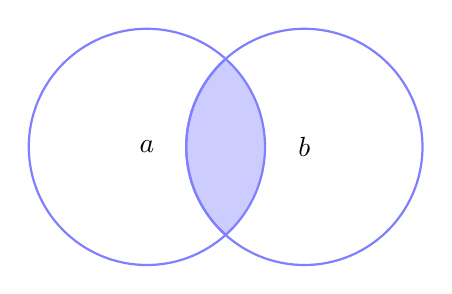
\begin{tikzpicture}
		\begin{scope}
			\clip \firstcircle;
			\fill[filled] \secondcircle;
		\end{scope}
		\draw[outline] \firstcircle node {$a$};
		\draw[outline] \secondcircle node {$b$};
	\end{tikzpicture}
	\captionof{figure}{$a \cap b$}
\end{center}

\begin{example}
	\begin{enumerate}
	\item Si considerino gli insiemi $a=\{3,4,5,6\}$ e $b=\{3,4,6,7\}$. Si avrà:
	\begin{displaymath}
		a \cap b = \{3,4,6\}
	\end{displaymath}
\item Sia $V=\{2,4,6,...\}$ l'insieme dei multipli di 2, mentre $W=\{3,6,9,...\}$ l'insieme dei multipli di 3. Allora:
\begin{align*}
	V \cap W = \{6,12,18,...\}
\end{align*}
Ossia l'insieme dei multipli di 6.
	\end{enumerate}
\end{example}
\begin{osservation}
\begin{enumerate}
	\item $a \cap b$ è contenuto, quale sottoinsieme, tanto in $a$ che in $b$:
	\begin{align*}
		(a \cap b) \subseteq a \land (a \cap b) \subseteq b
	\end{align*}

	\item Se due insiemi non hanno elementi comuni, se in altri termini, $a \cap b = \emptyset$, allora si dice che i due insiemi sono \textbf{disgiunti}.
\end{enumerate}
\end{osservation}

\subsection{Unione}
\dfn{Unione}{\index{Unione}
	Siano $a$, $b$ insiemi. Si definisce \textbf{unione} tra $a$ e $b$ l'insieme così definito:
	\begin{equation}
		a \cup b = \{x| x \in a \lor x \in b\}
	\end{equation}
}

\begin{center}
	\def\firstcircle{(0,0) circle (1.5cm)}
	\def\secondcircle{(0:2cm) circle (1.5cm)}
	\colorlet{circle edge}{blue!50}
	\colorlet{circle area}{blue!20}
	\tikzset{filled/.style={fill=circle area, draw=circle edge, thick},
		outline/.style={draw=circle edge, thick}}
	\setlength{\parskip}{5mm}
	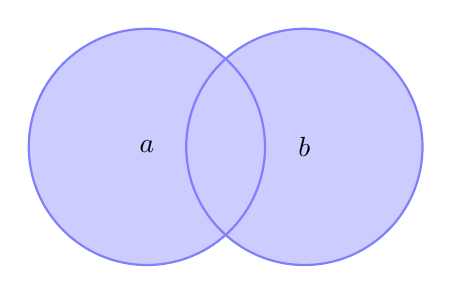
\begin{tikzpicture}
		\draw[filled] \firstcircle node {$a$}
		\secondcircle node {$b$};
	\end{tikzpicture}
	\captionof{figure}{$a \cup b$}
\end{center}

\begin{example}
 Si considerino gli insiemi $a=\{3,4,5,6\}$ e $b=\{3,4,6,7\}$. Si avrà:
	\begin{displaymath}
		a \cup b = \{3,4,5,6,7\}
	\end{displaymath}
\end{example}
\begin{osservation}
Tanto $a$ quanto $b$ sono sempre sottoinsiemi di $a \cup b$, ossia:
	\begin{align*}
		a \subset (a \cup b) \land b \subset (a \cup b)
	\end{align*}
\end{osservation}

Dato un insieme $a=\{x \; | \; \varphi(x)\}$ e $b=\{y \; | \; \psi(y)\}$, le operazioni insiemistiche appena viste possono essere tradotte con i connettivi logici applicati ai predicati dei relativi insiemi. Si avrà quindi:
\begin{eqnarray*}
	a \cap b \iff \varphi \land \psi \\
	a \cup b \iff \varphi \lor \psi
\end{eqnarray*}
Dalle tautologie d'idempotenza, commutatività e associatività (Vedi \ref{proprietà_connettivi}) e le leggi distributive per $\land$ e $\lor$ si ottengono le analoghe proprietà per le operazioni di unione e intersezione tra insiemi.

\begin{propbox}
	Per ogni insieme $a$, $b$, $c$ valgono le seguenti proprietà:
	\begin{eqnarray}
		a=a \cap a, \qquad a\cap b=b\cap a, \qquad a\cap(b \cap c) = (a \cap b ) \cap c, \\
		a=a \cup a, \qquad a\cup b=b\cup a, \qquad a\cup(b \cup c) = (a \cup b ) \cup c
	\end{eqnarray}
	che esprimono l'\textbf{idempotenza}, la \textbf{commutatività} e l'\textbf{associatività} delle operazioni di intersezione ed unione. Si hanno inoltre:
	\begin{eqnarray} \label{prop:distributivaunioneintersezione}
		a \cap (b \cup c) = (a \cap b) \cup (a \cap c) \\
		a \cup (b \cap c) = (a \cup b) \cap (a \cup c)
	\end{eqnarray}
	che esprimono le proprietà distributive dell'unione rispetto all'intersezione e viceversa.
\end{propbox}

\subsection{Differenza insiemistica}

\dfn{Differenza insiemistica}{
	\index{Differenza}
	Siano $a$, $b$ due insiemi. Si definisce \textbf{sottrazione} tra $a$ e $b$ e si indica con  $a \setminus b$ l'insieme: 
	\begin{equation}
		a \setminus b = \{x \in a \; | \; x \notin b \}
	\end{equation}
}
\begin{center}
	\def\firstcircle{(0,0) circle (1.5cm)}
	\def\secondcircle{(0:2cm) circle (1.5cm)}
	\colorlet{circle edge}{blue!50}
	\colorlet{circle area}{blue!20}
	\tikzset{filled/.style={fill=circle area, draw=circle edge, thick},
		outline/.style={draw=circle edge, thick}}
	\setlength{\parskip}{5mm}
\begin{minipage}{.45\textwidth}
	\centering
		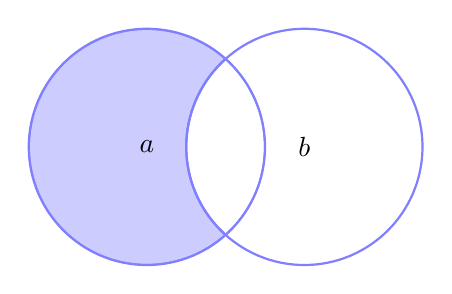
\begin{tikzpicture}
		\begin{scope}
			\clip \firstcircle;
			\draw[filled, even odd rule] \firstcircle node {$a$}
			\secondcircle;
		\end{scope}
		\draw[outline] \firstcircle
		\secondcircle node {$b$};
	\end{tikzpicture}
	\captionof{figure}{$a \setminus b$}
\end{minipage}
\begin{minipage}{.45\textwidth}
	\centering
			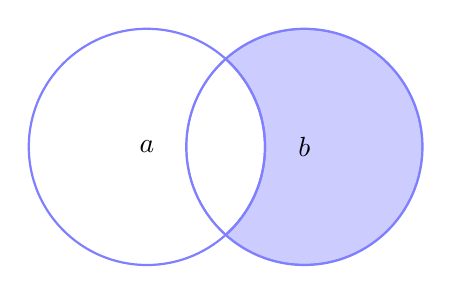
\begin{tikzpicture}
			\begin{scope}
				\clip \secondcircle;
				\draw[filled, even odd rule] \firstcircle
				\secondcircle node {$b$};
			\end{scope}
			\draw[outline] \firstcircle node {$a$}
			\secondcircle;
		\end{tikzpicture}
		\captionof{figure}{$b \setminus a$}
\end{minipage}
\end{center}
\begin{osservation}
	L'insieme $a$ contiene $a \setminus b$ come sottoinsieme:
	\begin{align*}
		a \setminus b \subset a
	\end{align*}

	Se l'insieme $a$ è parte di $b$ allora:	$$b \setminus a = \{x \in b | x \notin a\}$$
	Posto con $\alpha$ la condizione di appartenenza all'insieme $a$ (  $\alpha(x) \iff x \in a$), possiamo riscrivere la differenza precedente come segue: $$b \setminus a = \{x \in b | \neg \alpha \}$$	
Dalla tautologia della doppia implicazione si può ricavare una proprietà interessante:
\begin{align}\label{differenza_prop1}
	b \setminus (b \setminus a) &= \{x \in b | \neg (\neg \alpha)\} \nonumber \\
	&= \{x \in b \; | \; x \in a\} \nonumber \\
	&= a
\end{align}
\end{osservation}
L'osservazione precedente, chiaramente, non vale in generale per qualsiasi insieme $a$ e $b$ ma solo nel caso in cui $a$ sia sottoinsieme di $b$. Infatti, posto ``$\alpha= x \in a$'' e ``$\beta= x \in b$'' si ha, per ogni $a,b$:
\begin{align*}
	a \setminus (a \setminus b) = \Biggl\lbrace x | \alpha \land \Bigl(\neg \bigl(\alpha \land (\neg \beta) \bigr) \Bigr) \Biggr \rbrace &\iff  \Biggl\lbrace x | \alpha \land \Bigl((\neg \alpha) \lor \bigl(\neg(\neg \beta)\bigr)\Bigr) \Biggr \rbrace \\
	&\iff \Bigl \lbrace x | \alpha \land \bigl((\neg \alpha) \lor \beta\bigr)\Bigr \rbrace \\
	&\iff \Bigl\lbrace x |\bigl(\alpha \land (\neg \alpha)\bigr) \lor (\alpha \land \beta) \Bigr \rbrace \\
	&\iff \{x | \alpha \land \beta\} =  a \cap b
\end{align*}

Dati $n$ insiemi, un diagramma di Eulero Venn generico deve poter delimitare in maniera univoca ciascun tipo di intersezione per ogni insieme rappresentato. Ad esempio, supponendo di avere a disposizione cinque insiemi $a$, $b$, $c$, $d$ ed $e$, il diagramma di Eulero Venn mostrato in Figura \ref{fig:notvenn} non risulta essere un diagramma generico in quanto non sono rappresentate tutte le possibili intersezioni tra gli insiemi.
\begin{center}
	\begin{minipage}{.45\textwidth}
		\centering
		\includegraphics[scale=.35]{res/Not_Venn}
		\captionof{figure}{}\label{fig:notvenn}
	\end{minipage}
	\hfill
	\begin{minipage}{.45\textwidth}
		\centering
		\includegraphics[scale=.25]{res/Venn}
		\captionof{figure}{}\label{fig:venn}
	\end{minipage}
\end{center}

\subsection{Le leggi di De Morgan e differenza simmetrica}
\begin{teorbox}
	Siano $a$, $b$, $c$ insiemi. Valgono allora le seguenti formule che prendono il nome di \textbf{leggi di De Morgan}:
	\begin{eqnarray}
		a \setminus (b \cap c) = (a \setminus b ) \cup (a \setminus c) \\
		a \setminus (b \cup c) = (a \setminus b) \cap (a \setminus c) \label{eq:demorgan2}
	\end{eqnarray}
\end{teorbox}

\begin{proof}
	Siano $\alpha,\beta,\gamma$ i predicati di appartenenza nella variabile $x$, rispettivamente: $\alpha$ è ``$x \in a$", $\beta$ è ``$x \in b$", $\gamma$ è ``$x \in c$". Da queste definizioni segue:
	\begin{align*}
		x \in a \setminus (b \cap c) &\iff \alpha \land \bigl(\neg (\beta \land \gamma)\bigr)  \\
		&\iff  \Bigl(\alpha \land \bigl((\neg \beta) \lor (\neg \gamma)\bigr)\Bigr)  \\
		&\iff  \Bigl(\bigl(\alpha \land (\neg \beta)\bigr) \lor \bigl(\alpha \land (\neg \gamma)\bigr)\Bigr)  \\
		&\iff  x \in (a \setminus b) \cup (a \setminus c)
	\end{align*}
	
	Similmente si dimostra l'equazione \ref{eq:demorgan2}.
\end{proof}


\dfn{Differenza simmetrica}{
	Si definisce l'operazione insiemistica $\triangle$ di \textbf{differenza simmetrica} l'operazione corrispondente alla disgiunzione esclusiva. Si pone dunque, per ogni insieme $a$ e $b$:
	\begin{equation}
		a \triangle b := \{ x \; | \; (x \in a) \xor (x \in b) \}
	\end{equation}
}


La tautologia che abbiamo chiamato \textbf{esplicitazione di XOR} (Vedi Formula \ref{eq:exclusive-or-2}) implica facilmente:
\begin{equation}
	a \triangle b = (a \setminus b) \cup (b \setminus a) = (a \cup b) \setminus (b \cap a)
\end{equation}
mentre la commutatività e l'associatività di $\xor$ e la distributività di $\land$ rispetto a $\xor$ forniscono la commutatività e l'associatività di $\triangle$ e la distributività di $\cap$ rispetto a $\triangle$. Per ogni insieme $a,b,c$ abbiamo cioè:
\begin{eqnarray}
	a \triangle b &=& b \triangle a \\
	a \triangle(b \triangle c) &=& (a \triangle b) \triangle c \\
	a \cap ( a \triangle c) &=& (a \cap b) \triangle (a \cup c)
\end{eqnarray}
\begin{center}
	% Definition of circles
	\def\firstcircle{(0,0) circle (1.5cm)}
	\def\secondcircle{(0:2cm) circle (1.5cm)}
	\colorlet{circle edge}{blue!50}
	\colorlet{circle area}{blue!20}
	\tikzset{filled/.style={fill=circle area, draw=circle edge, thick},
		outline/.style={draw=circle edge, thick}}
	\setlength{\parskip}{5mm}
	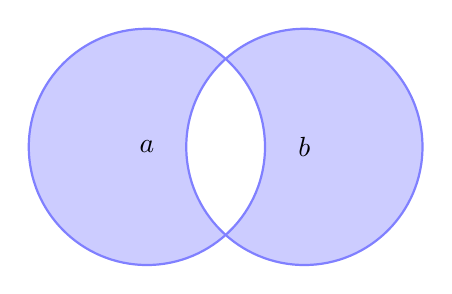
\begin{tikzpicture}
		\draw[filled, even odd rule] \firstcircle node {$a$}
		\secondcircle node{$b$};
	\end{tikzpicture}
	\captionof{figure}{$a \triangle b$}
\end{center}
\subsection{Operazioni unarie}
Per ogni insieme $s$ abbiamo definito l'insieme delle parti come l'insieme di tutti i sottoinsiemi di $s$. Dato però un numero naturale $n$ è possibile definire un altro insieme delle parti che va sotto il nome di \textbf{insieme delle parti $n$-arie}.

\dfn{Insieme delle parti $n$-arie}{
	Per ogni numero naturale $n \in \mathbb{N}$ e per ogni insieme $s$ si ha:
	\begin{equation}
		\mathcal{P}_{n}(s) = \biggl\{x \; | \; x \subseteq s \wedge \mbox{$x$  ha esattamente $n$ elementi}\biggr\}
	\end{equation}
}

\begin{example}
	Dato un insieme $s$ si ha $\mathcal{P}_{0}(s)= \{ \varnothing \} $ e $\mathcal{P}_{1}(s)= \bigl\{ \{x\} \; | \; x \in s \bigr\}$.
\end{example}

\dfn{Unione unaria}{
	Sia $a$ un insieme. Si definisce \textbf{unione unaria} di $a$ e si denota col simbolo $\bigcup a$ l'insieme:
	\begin{equation}
		\bigcup a = \{ x \; | \; \exists y \in a (x \in y)\}
	\end{equation}
	ovvero l'\textit{insieme degli elementi dei sottoinsiemi di $a$}.
}

\begin{example}
\begin{enumerate}
	\item Per ogni $m \in \mathbb{N}$ si pone:
\begin{displaymath}
	I_{m} = [0,m] = \{ x \in \mathbb{R} \; | \; 0 \leq x \leq m \}
\end{displaymath}
per definire un \textbf{intervallo chiuso reale} di estremi $0$ ed $m$. Denotiamo con $a= \{I_{m} \; | \; m \in \mathbb{N} \}$ l'insieme di tutti gli intervalli siffatti. Allora l'unione unaria di $a$ sarà:
\begin{displaymath}
	\bigcup a = \{x \in \mathbb{R} | x \geq 0 \} = \mathbb{R}^{+}
\end{displaymath}
\item Sia $S = \{\{1,5,7\},\{1,5,8,9\},\{2,15,66\}\}$, allora è:
\begin{displaymath}
	\bigcup S = \{1,2,5,7,8,9,15,66\}
\end{displaymath}
\end{enumerate}
\end{example}


\begin{example}
	L'unione unaria delle parti di $\mathbb{N}$ è $\mathbb{N}$ stesso. Infatti, preso un qualsiasi numero naturale è possibile prendere un sottoinsieme che lo contiene:
	\begin{displaymath}
		\forall n \in \mathbb{N} \bigl(\exists b \in \mathcal{P}(\mathbb{N})(n \in b)\bigr)
	\end{displaymath}
	Questo vuol dire allora che $\mathbb{N}$ è un sottoinsieme dell'unione unaria dell'insieme delle sue parti: $$\mathbb{N} \subseteq \bigcup \mathcal{P}(\mathbb{N})$$
	
	Per la definizione di inclusione (Formula \ref{eq:inclusione}) questo vuol dire che:
	\begin{displaymath}
		\forall x \bigl( x \in \mathbb{N} \implies x \in \bigcup \mathcal{P}(\mathbb{N}) \bigr)
	\end{displaymath}
	Preso un numero $y \notin \mathbb{N}$ ci chiediamo se questo possa appartenere a $\bigcup \mathcal{P} (\mathbb{N})$. Per appartenere a tale insieme deve soddisfare alla condizione:
	\begin{displaymath}
		y \in \bigcup \mathbb{N} \iff (\exists b \in \mathcal{P}(\mathbb{N})(y \in b))
	\end{displaymath}
	Il che è chiaramente falso in quanto abbiamo ipotizzato che $y$ non sia un numero naturale. Quindi possiamo dire che $\forall x \bigl( x \notin \mathbb{N} \implies x \notin \bigcup \mathcal{P}(\mathbb{N}) \bigr)$. Dalla \hyperlink{contrapposizione}{legge di contrapposizione} si ha quindi:$$\forall x (x \in \bigcup \mathcal{P}(\mathbb{N}) \implies x \in \mathbb{N})$$ Ovvero $\bigcup \mathcal{P}(\mathbb{N}) \subseteq \mathbb{N}$. e allora $\mathbb{N} = \bigcup \mathcal{P}( \mathbb{N})$ per la legge della doppia inclusione (Formula \ref{eq:doppia_inclusione}).
\end{example}

\dfn{Intersezione unaria}{
	Sia $a \neq \varnothing$ un insieme non vuoto. Si definisce \textbf{intersezione unaria} di $a$ e si denota col simbolo $\bigcap a$ l'insieme:
	\begin{equation}
		\bigcap a = \{x \; | \; \forall b \in a (x\in b)\}
	\end{equation}
	ovvero l'\textit{insieme degli elementi che appartengono a ciascun elemento di $a$}.
}


\begin{osservation}
\begin{enumerate}
	\item È importante precisare che $a$ non possa essere l'insieme vuoto altrimenti si avrebbe una contraddizione. Infatti:
	\begin{displaymath}
		\bigcap \varnothing = \{x | \forall y \in \varnothing (x \in y)\}
	\end{displaymath}
	il che rappresenterebbe l'insieme di tutti gli insiemi.
	
	\item Sia $c=\{a,b\}$ un insieme contenente gli insiemi $a$ e $b$. Quindi, per definizione di unione unaria si ha che $\bigcup c$ è l'insieme degli elementi che si trovano o in $a$ o in $b$:
	\begin{displaymath}
		\bigcup c = \{x \; | \; \exists y \in c (x \in y)\} = \{x \; | \; x \in a \vee x \in b\} = a \cup b
	\end{displaymath}
	Quindi l'unione tra due insiemi altro non è che un caso particolare dell'unione unaria applicato ad un insieme formato da due elementi. Grazie all'operazione unaria è possibile quindi effettuare unioni tra infiniti oggetti. Analogamente per l'intersezione unaria $\bigcap \{a,b\} = a \cap b$.
\end{enumerate}
\end{osservation}

\begin{propbox}[Formule generalizzate di associatività, distributività e di De Morgan]
	Per ogni $a,b$ insiemi non vuoti valgono:
	\begin{eqnarray}
		(\bigcap a) \cap (\bigcap b) = \bigcap (a \cup b) \\
		(\bigcap a) \cup (\bigcap b) = \bigcup (a \cap b )\\
		a \cap (\bigcup b) = \bigcup_{x \in b} (a \cap x) \\
		a \cup (\bigcap b) = \bigcap_{x \in b} (a \cup x)\\
		a \setminus \bigcup b = \bigcap_{x \in b} ( a \setminus x) \\
		a \setminus \bigcap b = \bigcup_{x \in b} (a \setminus x)
	\end{eqnarray}
\end{propbox}

\begin{proof} 
	La dimostrazione di queste formule è lasciata al lettore come esercizio.
\end{proof}

\section{Prodotto Cartesiano di Insiemi}

\subsection{Coppie ordinate}

\dfn{Coppia ordinata}{\index{Coppia ordinata}
	Siano $a$, $b$ insiemi. Una \textbf{coppia ordinata} si denota col simbolo $(a,b)$ e gode della seguente proprietà:
	\begin{equation}
		\forall \ a,b,c,d \qquad (a,b)=(c,d) \Longleftrightarrow (a=c \wedge b=d)
	\end{equation}
}

\begin{propbox}
	Per ogni $a,b,c,d$ si ha:
	\begin{displaymath}
		\{\{a\}, \{a,b\}\} = \{\{c\}, \{c,d\}\} \iff a = c \wedge b = d
	\end{displaymath}
\end{propbox}

\begin{proof}
	($\implies$) Si supponga quindi che $\{\{a\}, \{a,b\}\} = \{\{c\}, \{c,d\}\}$. Per l'assioma di estensionalità (Assioma \ref{axiom:extensionality}) allora entrambi gli insiemi hanno gli stessi elementi. Se $a=b$ allora $\{\{a\},\{a,b\}\}=\{\{a\}\}$ ha un solo elemento, per cui anche $\{\{c\},\{c,d\}\}$ ha un solo elemento. Quindi $a=b=c=d$.
	
	Sia allora $a \neq b$. Dall'ipotesi $\{\{a\}, \{a,b\}\} = \{\{c\}, \{c,d\}\}$ segue allora $c \neq d$, per cui deve essere:
	\begin{eqnarray*}
		\{a\}=\{c\} &\implies& a=c \\
		\{a,b\}=\{c,d\} &\implies& b=d
	\end{eqnarray*}
	
	($\impliedby$) Chiaramente la condizione è sufficiente.
\end{proof}

Si può usare questa proposizione per dare una definizione esplicita delle coppie ordinate, ponendo: $$\forall a,b \qquad (a,b) \coloneqq \{\{a\}, \{a,b\}\}$$  Questa è la cosiddetta \textbf{definizione di Kuratowski} della nozione di coppia ordinata.

\subsection{Prodotti cartesiani}

\dfn{Prodotto cartesiano}{\index{Prodotto cartesiano}
	Siano $a$, $b$ insiemi. Si dice \textbf{prodotto cartesiano} di $a$ e $b$, e si denota col simbolo $a \times b$, l'insieme di tutte le coppie $(x,y)$, con $x$ appartenente ad $a$ e $y$ appartenente a $b$.
	\begin{equation}
		a \times b = \bigl \{(x,y) \; | \; x \in a \wedge y \in b \bigl \}
	\end{equation}
}


\begin{example}
	Ad esempio se $a=\{1,2,3\}$ e $b=\{1,2\}$, allora $$a \times b=\{(1,1),(2,1),(3,1),(1,2),(2,2),(3,2)\}$$
	\begin{center}
		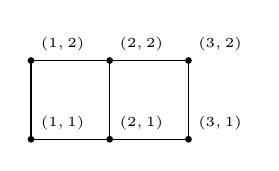
\begin{tikzpicture}
			\draw[step=1.0,black,thin] (1,1) grid (3,2);
			\foreach \x in {1,...,3}
			\foreach \y in {1,2}
			\filldraw (\x,\y) circle[radius=1pt] node[above right] {\tiny $(\x,\y)$};
		\end{tikzpicture}
	\end{center}
\end{example}

\dfn{Terna ordinata}{\index{Terna ordinata}
	Si definisce una \textbf{terna ordinata} $(a,b,c)$ come una coppia ordinata in cui la prima coordinata è una coppia ordinata $(a,b)$ e come seconda coordinata $c$:
	\begin{equation}
		\forall a,b,c \qquad (a,b,c) = \bigl((a,b),c\bigr)
	\end{equation}
}

\begin{propbox}\label{prop_terne_ordinate}
	Due terne ordinate $(a,b,c)$ e $(d,e,f)$ sono uguali se e solo se:
	\begin{equation}
		\forall a,b,c,d,e,f \qquad \bigl((a,b),c\bigr) = \bigl((d,e),f\bigr) \iff (a=d \wedge b=e \wedge c=f)
	\end{equation}
\end{propbox}

\begin{proof}
	L'enunciato si dimostra facilmente ponendo $(a,b)=m$ e $(d,e)=n$. In questo modo la dimostrazione si riduce alla dimostrazione già vista delle coppie ordinate $(m,c)$ e $(n,f)$. 
\end{proof}
\newpage
\section{Esercizi svolti}
\begin{exsbox}
	Verificare $3 \in \{2n^{2}+1 \; | \; n \in \mathbb{Z}\}$.
\end{exsbox}
\paragraph{Svolgimento.} Poniamo $A=\{2n^{2}+1 / n \in \mathbb{Z}\}$. Per essere verificata l'appartenenza deve valere la seguente equivalenza logica
\begin{displaymath}
	3 \in A \iff \exists n \in \mathbb{Z}(3=2n^{2}+1)
\end{displaymath}
e procediamo sviluppando algebricamente tale relazione fino ad ottenere una relazione più semplice da valutare:
\begin{align*}
	3 \in A &\iff \exists n \in \mathbb{Z}(3=2n^{2}+1)\\
	&\iff \exists n \in \mathbb{Z}(2=2n^{2}) & \text{\textcolor{gray}{Spostando 1 a sinistra}}\\
	&\iff \exists n \in \mathbb{Z}(n^{2}=1) & \text{\textcolor{gray}{Semplificando}}
\end{align*}
L'ultima equivalenza è chiaramente vera in quanto, per $n=\pm 1 \in \mathbb{Z}$ si ha $n^{2}=1$. Quindi $3 \in A$. \hfill \blacksquare
\begin{exsbox}
	Sia $A= \{\{a,b\}/a,b \in \mathbb{Z}\}$ un insieme. Verificare $\{1\} \in A$ e $\{1,2,3\} \in A$.
\end{exsbox}
\paragraph{Svolgimento.} Chiaramente:
\begin{align*}
	\{1\} \in A \iff \exists a,b \in \mathbb{Z}(\{a,b\} = \{1\})
\end{align*}
che risulta vera per $a=b=1$. Infatti $\{1,1\}=\{1\} \in A$. Al contrario, non esistono due numeri interi relativi tali che $\{a,b\}=\{1,2,3\}$ in quanto tale insieme contiene 3 elementi mentre $\{a,b\}$ ne può contenere al massimo due (quando $a \neq b$). Quindi $\{1,2,3\} \notin A$. \hfill \blacksquare
\begin{exsbox}
	Sia $f=\{\{a,b\},\{b,d\}\}$. Si calcolino $\bigcap f$ e $\bigcup f$.
\end{exsbox}
\paragraph{Svolgimento.} L'intersezione unaria di $f$ è definita come l'insieme degli elementi appartenenti a ciascun elemento di $f$, ovvero:
\begin{displaymath}
	\bigcap f = \{x / \forall y \in f (x \in y)\} = \{a,b\} \cap \{b,d\}= \{b\}
\end{displaymath}
\marker{yellow!50}{yellow!20!black}{Non dimenticare che $b \neq \{b\}$, nel primo caso ci si sta riferendo all'entità $b$ mentre nel secondo al singleton dell'entità $b$. \emph{Sarebbe stato un errore} scrivere quindi $\bigcap f = b$.}
Nel caso dell'unione unaria abbiamo che:
\begin{displaymath}
	\bigcup f = \{x / \exists y \in f (x \in f)\} = \{a,b\} \cup \{b,d\} = \{a,b,d\}
\end{displaymath}
\hfill \blacksquare
\begin{exsbox}
	Sia $A$ l'insieme dei numeri pari e $B$ quello dei numeri naturali moltiplicati per 2; dire in quale relazione stanno i due insiemi.
\end{exsbox}
\paragraph*{Svolgimento.} Per definizione di numero pari esprimiamo l'insieme $A$ come: $$\{p \in \mathbb{Z} / \exists k \in \mathbb{Z}(p = 2k)\}$$ mentre $$B= \{m \in \mathbb{N} / \exists k \in \mathbb{N} (m = 2k) \}$$ Ovviamente vale $B \subset A$. \hfill \blacksquare
\begin{exsbox}
	Decidere se esistono e, nel caso, descrivere esplicitamente gli insiemi:
	\begin{enumerate}
		\item $\{x | \forall y(x=y) \} $
		\item $\{ x|\forall y(x \neq y) \}$
		\item $ \{ x| \exists y (x=y)\}$
		\item $\{x|\exists y(x \neq y)\}$
		\item $ \{ x| \forall y (y \subseteq x) \}$
		\item $\{x|x=\{0,1,2\} \}$
		\item $\{y|y=\{0,1,2\} \}$
		\item $\{ x | x= \{0,1,2,x \} \}$
	\end{enumerate}
\end{exsbox}
\paragraph*{Svolgimento.} Si ha:
\begin{enumerate}
	\item  $\{x | \forall y(x=y) \} = \varnothing$. Non esiste infatti un insieme $x$ che sia uguale a tutti gli insiemi $y$. Quindi non esiste nessun elemento in questo insieme. Quindi l'insieme è l'insieme vuoto.
	\item $\{x|\forall y(x \neq y)\}= \varnothing$. Infatti non è vero che per ogni $x$, comunque si prenda un insieme $y$ allora $x \neq y$ perché appunto si potrebbe scegliere $x$ stesso al posto di $y$ ottenendo la proposizione ``$\forall x(x \neq x)$'' e poiché ogni oggetto è uguale a stesso allora si può dire che non esistono oggetti che appartengono alla totalità descritta dalla formula e per questo motivo l'insieme descrive l'insieme vuoto.
	\item Va notato che la proprietà di questo insieme è la negazione dell'insieme precedente. Per questo motivo possiamo dire che la proprietà è vera in quanto è vero che esiste almeno un insieme tale per cui sia uguale ad $x$ (ovvero $x$ stesso). Essendo vera questa formula allora sarebbe vero che per ogni insieme $x$ questo appartiene all'insieme $A=\{x|\exists y(x=y)\}$ ma non esistendo l'insieme di tutti gli insiemi allora l'insieme in questione non esiste.
	\item Analogamente come nell'esercizio precedente.
	\item L'insieme $\{x|\forall y(y \subseteq x)\}$ rappresenta l'insieme vuoto. Infatti non esiste un insieme tale per cui, comunque si scelga un insieme $y$, esso sia parte di $x$. Per fugare ogni dubbio, per rendere evidente che questa proposizione è false basta trovare un controesempio: preso l'insieme $x$ è immediato osservare che il singleton $\{x\}$ non è contenuto in $x$:$\forall x \bigl(\{x\} \nsubseteq x \bigr)$.
	\item L'insieme $\{x|x=\{0,1,2\}\}$ esiste ed ha un solo elemento. Infatti, per l'assioma di estensionalità, l'insieme delle $x$ tali che $x=\{0,1,2\}$ è il singleton di siffatto insieme $x$. Quindi:
	\begin{displaymath}
		\{x|x=\{0,1,2\}\} = \bigl\{ \{0,1,2\}  \bigr\}
	\end{displaymath}
	\item Uguale all'insieme precedente.
	\item $A=\{x|x=\{0,1,2,x\}\}=\varnothing$. Infatti si deve avere $\forall x(x \in A \iff \varphi)$, dove $\varphi$ rappresenta il predicato ``$x=\{0,1,2,x\}$''. Questa condizione è falsa per ogni $x$ in quanto nessun insieme appartiene a sé stesso e quindi l'insieme $A$ è vuoto. \hfill \blacksquare
\end{enumerate}
\begin{exsbox}
	Dire quali delle seguenti relazioni sono vere e quali false:
	\begin{enumerate}
		\item $\{1,3,5,10\} = \{3,1,10,5\}$;
		\item $\{a,b,d\}=\{b,d,a\}$;
		\item $\{2,5,6\} = \{2,7,5\}$;
		\item $\{a\} = a$;
		\item $a \in \{a\}$;
	\end{enumerate}
\end{exsbox}
\paragraph{Svolgimento.} Si ha:
\begin{enumerate}
	\item Vero
	\item Vero
	\item Falso
	\item Falso
	\item Vero \hfill \blacksquare
\end{enumerate}
\begin{exsbox}
	Sia $x=\{\{\{\{\varnothing\}\}\}\}$. Quanti elementi ha $x$? Quante parti ha $x$?
\end{exsbox}
\paragraph{Svolgimento.} L'insieme $x$ ha un solo elemento, di conseguenza l'insieme delle parti avrà solo le parti banali. \hfill \blacksquare
\begin{exsbox}
	Vero o falso?
	\begin{enumerate}
		\item $\varnothing \in \varnothing$
		\item $\varnothing \subseteq \varnothing$
		\item $\varnothing \subset \varnothing$
		\item $\varnothing \in \mathcal{P}(\varnothing)$
		\item $\varnothing \subseteq \mathcal{P}(\varnothing)$
		\item $\varnothing = \{\varnothing\}$
		\item $\varnothing \subseteq \{\varnothing\}$
		\item $\varnothing \in \{\varnothing\}$
		\item $\{1,1,2,2,2,3,3\}$ è una parte di $\{2,1,3\}$
		\item $\{1,1,2,2,2,3,3\}$ è una parte di $\{4,2,1,3\}$
	\end{enumerate}
\end{exsbox}
\paragraph{Svolgimento.} Si ha:
\begin{enumerate}
	\item Falso
	\item Vero
	\item Falso
	\item Vero
	\item Vero
	\item Falso
	\item Vero
	\item Vero
	\item Vero
	\item Vero. \hfill \blacksquare
\end{enumerate}
\begin{exsbox}
	Elencare gli elementi di $\mathcal{P}(\{0,1,2\})$.
\end{exsbox}
\paragraph{Svolgimento.}
Si ha $\mathcal{P}(\{0,1,2\})=\bigl\{ \varnothing, \{0,1,2\},\{ 0\},\{1\},\{2\},\{1,2\},\{0,1\},\{0,2\}   \bigr\} $.
\hfill \blacksquare

\begin{exsbox}
	Illustrare con i grafici di Eulero Venn la proprietà transitiva dell'inclusione tra i seguenti insiemi:
	\begin{displaymath}
		\begin{array}{lll}
			A = \{2,3,5\} & B= \{2,3,8,5\} & C = \{3,2,8,5,10,12\}
		\end{array}
	\end{displaymath}
\end{exsbox}
\paragraph{Svolgimento.} Si ha:
\begin{center}
	\includegraphics[scale=.45]{res/Venn_Esercizio1}
\end{center}
\hfill \blacksquare
\begin{exsbox}
	Determinare rispetto a $\mathbb{Z}$ gli insiemi complementari dei seguenti insiemi:
	\begin{enumerate}
		\item $\{x / x \in \mathbb{Z} \land x <3\}$
		\item $\{x / x \in \mathbb{Z} \land 2 \leq x \leq 5 \}$
		\item $\{x / x \in \mathbb{Z} \land 1 < x < 5 \}$
		\item $\{x / x \in \mathbb{Z} \land 1 \leq x \leq 2 \}$
		\item $\{x / x \in \mathbb{Z} \land x \geq 1 \}$
		\item $\{x / x \in \mathbb{Z} \land x \leq 0 \}$
	\end{enumerate}
\end{exsbox}
\paragraph{Svolgimento.} Definiamo complemento di una parte $X$ di un insieme non vuoto $S$ la differenza $S \setminus X$. Abbiamo allora:
\begin{enumerate}
	\item $\mathbb{Z} \setminus \{x / x \in \mathbb{Z} \land x <3\} = \{x / x \in \mathbb{Z} \land x > 3\}$;
	\item $\mathbb{Z} \setminus \{x / x \in \mathbb{Z} \land 2 \leq x \leq 5 \} = \{x / x \in \mathbb{Z} \land x < 2 \land x > 5\}$;
	\item $\mathbb{Z} \setminus \{x / x \in \mathbb{Z} \land 1 < x < 5 \} = \{x / x \in \mathbb{Z} \land x \leq 1 \land x \geq 5\}$;
	\item $\mathbb{Z} \setminus \{x / x \in \mathbb{Z} \land 1 \leq x \leq 2 \} = \{x /  x \in \mathbb{Z} \land x < 1 \land x > 2\}$;
	\item $\mathbb{Z} \setminus \{x / x \in \mathbb{Z} \land x \geq 1 \} = \{x / x \in \mathbb{Z} \land x < 1 \}$;
	\item $\mathbb{Z} \setminus \{x / x \in \mathbb{Z} \land x \leq 0 \} = \{x / x \in \mathbb{Z} \land x > 0 \}$. \hfill \blacksquare
\end{enumerate}
\begin{exsbox}
	L'insieme $\mathbb{Z}$ appartiene a $\mathcal{P}(\mathbb{Z})$?
\end{exsbox}
\paragraph{Svolgimento.} Sì. In ogni insieme $S \neq \emptyset$ si ha che $\emptyset$ ed $S$ sono parti banali e appartengono a $\mathcal{P}(S)$. \hfill \blacksquare
\begin{exsbox}
	Descrivere esplicitamente gli insiemi:
	\begin{enumerate}
		\item $\{x | \forall y (x \cap y = \varnothing)\}$
		\item $\{x | \exists y (x \cup y = \varnothing)\}$
		\item $\{x | \forall y (x \cup y = \varnothing)\}$
	\end{enumerate}
\end{exsbox}
\paragraph{Svolgimento.} Si ha:
\begin{enumerate}
	\item $\{x | \forall y (x \cap y = \varnothing)\}=\{ \varnothing \}$. Infatti l'insieme rappresenta l'insieme degli insiemi che non hanno alcun elemento in comune con tutti gli insiemi. L'unico insieme a soddisfare questa proprietà è l'insieme vuoto.
	\item $\{x | \exists y (x \cup y = \varnothing)\} = \{ \varnothing\}$. Infatti l'insieme rappresenta l'insieme di tutti gli insiemi $x$ per i quali esiste almeno un insieme $y$ tale che l'unione con $x$ sia il vuoto. L'unico insieme a soddisfare tale proprietà è l'insieme vuoto in quanto $\varnothing \cup \varnothing = \varnothing$.
	\item $\{x | \forall y (x \cup y = \varnothing)\}= \varnothing$. Infatti non esiste un insieme per cui la sua unione con qualsiasi insieme sia uguale all'insieme vuoto. \hfill \blacksquare
\end{enumerate}
\begin{exsbox}
	Per quali coppie di insiemi $a$, $b$, si ha $a \setminus b = b \setminus a$?
\end{exsbox}
\paragraph{Svolgimento.} L'unico caso in cui $a \setminus b$ può essere uguale a $b \setminus a$ è quando $a=b$. Infatti si ha $a \setminus b = \varnothing = b \setminus a$. \hfill \blacksquare
\begin{exsbox}
	Rappresentare, in diagrammi di Venn generici, i termini insiemistici $a \setminus ( b \setminus c)$ e $(a \setminus b) \setminus c$. Decidere se è vera o falsa la proposizione: $(\forall a,b,c)(a \setminus(b \setminus c) = (a \setminus b) \setminus c)$. Ripetere l'esercizio per $a \cap (b \setminus c)$ e $(a \cap b)\setminus c$.
\end{exsbox}
\paragraph{Svolgimento.}
L'insieme $a\setminus(b\setminus c)$ è rappresentato dal diagramma di Venn \ref{fig:venn228} mentre l'insieme $(a\setminus b)\setminus c$ dal diagramma \ref{fig:venn2282}.
\begin{center}
	\begin{minipage}{.45\textwidth}
		\centering
		\includegraphics[scale=0.6]{res/path33251.png}
		\captionof{figure}{}\label{fig:venn228}
	\end{minipage}
	\hfil
	\begin{minipage}{.45\textwidth}
		\centering
		\includegraphics[scale=0.6]{res/path2879.png}
		\captionof{figure}{}\label{fig:venn2282}
	\end{minipage}
\end{center}
Osservando i due diagrammi possiamo concludere che la differenza simmetrica tra tre insiemi non gode della proprietà associativa. Non è vero dunque che:
$\forall \ a,b,c \Bigl(a \setminus (b\setminus c) = (a \setminus b) \setminus c \Bigr)$. Analogamente, i diagrammi di Eulero Venn \ref{fig:venn2283} e \ref{fig:venn2284} rappresentano gli insiemi $a\cap(b \setminus c)$ e $(a \cap b) \setminus c$.
\begin{center}
	\begin{minipage}{.45\textwidth}
		\centering
		\includegraphics[scale=0.5]{res/Venn2882.png}
		\captionof{figure}{}\label{fig:venn2283}
	\end{minipage}
	\hfil
	\begin{minipage}{.45\textwidth}
		\centering
		\includegraphics[scale=0.5]{res/Venn2882_2.png}
		\captionof{figure}{}\label{fig:venn2284}
	\end{minipage}
\end{center}
Dai due diagrammi ci si può convincere del fatto che: $\forall \ a,b,c \Bigl(a\cap(b \setminus c) = (a \cap b) \setminus c \Bigr)$. \hfill \blacksquare
\begin{exsbox}
	Rappresentare in diagramma di Eulero Venn $(a \triangle b) \triangle c$.
\end{exsbox}
\paragraph*{Svolgimento.}
Si ha che $(a \setminus b)\setminus c$ è uguale al seguente diagramma di Eulero Venn:
\begin{center}
	\includegraphics[scale=0.6]{res/diff3sim.png}
\end{center}

Infatti, posto $\alpha= x \in A$, $\beta=x \in B$ e $\gamma=x\in C$ si ha:
\begin{displaymath}
	x \in	(a \triangle b)\triangle c \iff \bigl( \alpha \xor \beta \bigr) \xor \gamma
\end{displaymath}
Che, per la tautologia \ref{eq:xor2} è equivalente all'implicazione:
\begin{displaymath}
	(\alpha \iff \beta) \iff \gamma
\end{displaymath}
che è vera quando vale una e una sola delle tre proprietà (come evidenziato dalle zone in verde alle estremità del diagramma) oppure valgono contemporaneamente (la parte centrale del diagramma).  \hfill \blacksquare

\begin{exsbox}
	Dimostrare che, per ogni $a$, $b$ sono equivalenti tra loro:
	\begin{enumerate}
		\item $a \subseteq b$
		\item $a \cap b = a$
		\item $a \cup b = b$
	\end{enumerate}
\end{exsbox}
\paragraph{Svolgimento.} ($1 \implies 2$) Dire che per ogni insieme $a$ e $b$ si ha $a \subseteq b$ significa affermare:
\begin{displaymath}
	\forall x (x \in a \implies x \in B)
\end{displaymath}
Poiché l'intersezione tra i due insiemi è l'insieme che contiene gli elementi in comune tra i due è evidente che l'insieme formato sia $a$.

($1 \implies 3$) Analogamente, se $a$ è un sottoinsieme di $b$ e l'unione è l'insieme formato da tutti gli elementi che si trovano o in $a$ o in $b$ allora l'unione tra i due insiemi è $b$ stesso.

($3 \implies 1$) Se $a \cup b = \{x | x \in a \lor x \in b\} = b$ può significare solo due cose. O che $a$ è l'insieme vuoto o che $a$ è un sottoinsieme di $b$. In entrambi i casi si ha $a \subseteq b$. \hfill \blacksquare

\begin{exsbox}
	Calcolare, per un arbitrario insieme $a$:
	\begin{enumerate}
		\item $a \triangle a$
		\item $a \triangle \emptyset $
	\end{enumerate}
\end{exsbox}
\paragraph{Svolgimento.} Per definizione di differenza simmetrica si ha:
\begin{align*}
	a \triangle a &= \{ x \; | \; x \in \bigl(( a \cup a) \setminus (a \cap a)\bigr) \}  \\
	&= \{x \; | \; x \in (a \setminus a) \} \\
	&= \varnothing
\end{align*}
mentre nel caso della seconda formula:
\begin{align*}
	a \triangle \varnothing &= \{ x \; | \; x \in \bigl(( a \cup \varnothing ) \setminus (a \cap \varnothing)\bigr) \} \\
	&= \{x \; | \; x \in (a \setminus \varnothing ) \} \\
	&= a
\end{align*}
\hfill \blacksquare

\begin{exsbox}
	Rappresentare, in un diagramma di Venn generico, il termine insiemistico $A \cap ( B \triangle C)$.
\end{exsbox}
\paragraph{Svolgimento. }Si procede calcolando innanzitutto $B \triangle C$ (la zona evidenziata di grigio) e poi si calcola l'intersezione con l'insieme $A$. Si ottiene così il diagramma di Venn mostrato in figura:
\begin{center}
	\includegraphics[scale=.6]{res/Venn_Esercizio2.png}
\end{center}
\hfill \blacksquare
\begin{exsbox}
	Rappresentare su un diagramma di Venn di tipo generale l'espressione insiemistica:
	$(A \setminus B) \triangle (B \cup C)$.
\end{exsbox}
\paragraph{Svolgimento.} Si ha:
\begin{align*}
	(A \setminus B) \triangle (B \cup C) &= \bigl((A \setminus B)  \cup (B \cup C)\bigr) \setminus \bigl((A \setminus B) \cap (B \cup C)\bigr) \\
\end{align*}
\begin{center}
	\includegraphics[scale=.6]{res/Venn_Esercizio3.png}
\end{center}
\hfill \blacksquare
\begin{exsbox}
	Rappresentare, in un diagramma di Venn generico, i termini insiemistici $A \cup (B \cap C)$ e $A \cap (B \cup C)$. Decidere se vale una delle formule:
	\begin{eqnarray}
		\forall A,B,C (A \cup (B \cap C) \subseteq A \cap (B \cup C))  \\
		\forall A,B,C (A \cup (B \cap C) \supseteq A \cap (B \cup C))
	\end{eqnarray}
\end{exsbox}
\paragraph{Svolgimento.}
Si ha $A \cup (B \cap C)$ rappresentato in figura \ref{fig:venn4} mentre $A \cap (B \cup C)$ è mostrato in Figura \ref{fig:venn5}.
\begin{center}
	\begin{minipage}{.45\textwidth}
		\centering
		\includegraphics[scale=.6]{res/Venn_Esercizio4.png}
		\captionof{figure}{$A \cup (B \cap C)$}\label{fig:venn4}
	\end{minipage}
	\hfil
	\begin{minipage}{.45\textwidth}
		\centering
		\includegraphics[scale=.6]{res/Venn_Esercizio5.png}
		\captionof{figure}{$A \cap (B \cup C)$}\label{fig:venn5}
	\end{minipage}
\end{center}
Osservando i diagrammi di Venn possiamo dire con certezza che $\forall A,B,C (A \cup (B \cap C) \supseteq A \cap (B \cup C))$. \hfill \blacksquare
\begin{exsbox}
	Rappresentare con un diagramma di Eulero Venn l'insieme: $\Bigl( \bigl(   (a \triangle b) \triangle c \bigr) \triangle d \Bigr)$.
\end{exsbox}
\paragraph{Svolgimento.} Affermare che un qualsiasi $x$ appartiene all'insieme $\Bigl( \bigl( (a \triangle b) \triangle c \bigr) \triangle d   \Bigr)$ è equivalente alla seguente catena di implicazioni:
\begin{align*}
	\forall x \biggl( x \in \Bigl( \bigl( (a \triangle b) \triangle c \bigr) \triangle d   \Bigr) \biggr) &\iff \forall x \Bigl( x \in \bigl( (a \triangle b) \triangle c \bigr) \xor (x \in d) \Bigr) \\
	&\iff \forall x \Bigl( \bigl( x \in (a \triangle b) \xor x \in c  \bigr) \xor (x \in d)        \Bigr) \\
	&\iff \forall x \Bigl( (x \in a) \xor (x \in b) \xor (x \in c) \xor (x \in d)   \Bigr)
\end{align*}
che è vera quando è vera singolarmente una delle condizioni di appartenenza oppure quando vale per tre di esse. Quindi l'insieme così ottenuto è quello evidenziato dalle strisce nel diagramma di Eulero Venn mostrato nella Figura \ref{fig:venn215}.
\begin{center}
	\includegraphics[scale=0.7]{res/path9768.png}
	\captionof{figure}{}\label{fig:venn215}
\end{center}
\begin{exsbox}
	Rappresentare, in diagrammi di Venn generici, i termini insiemistici $a \cap (b \triangle c)$ e $a \cup (b \triangle c)$, confrontandoli tra loro e con $(a \cap b) \triangle (a \cap c)$ e $(a \cup b) \triangle (a \cup c)$.
\end{exsbox}
\paragraph{Svolgimento.} Si ha:
\begin{center}
	\begin{minipage}{.45\textwidth}
		\centering
		\includegraphics[scale=.5]{res/Venn_Esercizio6.png}
		\captionof{figure}{$a \cap (b \triangle c)$}
	\end{minipage}
	\begin{minipage}{.45\textwidth}
		\centering
		\includegraphics[scale=.5]{res/Venn_Esercizio7.png}
		\captionof{figure}{$a \cup (b \triangle c)$}
	\end{minipage} \\
	\begin{minipage}{.45\textwidth}
		\centering
		\includegraphics[scale=.5]{res/Venn_Esercizio8.png}
		\captionof{figure}{$(a \cap b) \triangle (a \cap c)$}
	\end{minipage}
	\begin{minipage}{.45\textwidth}
		\centering
		\includegraphics[scale=.5]{res/Venn_Esercizio9.png}
		\captionof{figure}{$(a \cup b) \triangle (a \cup c)$}
	\end{minipage}
\end{center}
Osservando i vari diagrammi di Venn possiamo dire con certezza che vale:
\begin{displaymath}
	\begin{array}{l}
		a \cap (b \triangle c) = (a \cap b) \triangle (a \cap c)  \\
		a \cap (b \triangle c) \subset a \cup (b \triangle c) \\
		(a \cup b) \triangle (a \cup c) \subset  a \cup (b \triangle c)
	\end{array}
\end{displaymath}
\hfill \blacksquare
\begin{exsbox}
	Siano $a$ e $b$ due insiemi. Supposto $a \subseteq b$, descrivere $a \triangle b$.
\end{exsbox}
\paragraph{Svolgimento.} Per definizione
\begin{equation}\label{eq:diff_simm_parti}
	a \triangle b = (a \cup b) \setminus (a \cap b)
\end{equation}
Ma, essendo $a \subseteq b$, valgono le seguenti relazioni:
\begin{eqnarray}
	a \cup b = b \\
	a \cap b = a
\end{eqnarray}
Quindi, sostituendo tali relazioni in \ref{eq:diff_simm_parti} si ottiene:
\begin{align*}
	a \triangle b &= (a \cup b) \setminus (a \cap b) \\
	&= b \setminus a
\end{align*}
Ovvero il complemento di $a$ in $b$ come mostrato nel seguente diagramma di Venn:
\begin{center}
	\includegraphics[scale=.8]{res/Venn_Esercizio10}
\end{center}
\hfill \blacksquare
\begin{exsbox}
	Siano $A=\{n \in \mathbb{N} \; | \; 3 \leq n \leq 10\}$, $B$ l'insieme dei numeri naturali pari, $C=\{1,2,8,13,1234\}$. Descrivere, elencandone gli elementi:
	\begin{enumerate}
		\item $A\setminus B$
		\item $A \triangle C$
		\item $B \cap C$
		\item $B \triangle (B \setminus C)$.
	\end{enumerate}
\end{exsbox}
\paragraph{Svolgimento.} Abbiamo:
\begin{displaymath}
	\begin{array}{l}
		A \setminus B = \{3,5,7,9\}\\
		A \triangle C = \{1,2,4,5,6,7,9,10,13,1234\}\\
		B \cap C = \{2,8,1234\}\\
		B \triangle (B \setminus C) = \{2,8,1234\}
	\end{array}
\end{displaymath}
\marker{yellow!50}{yellow!20!black}{Sfrutta la proprietà della differenza simmetrica tra un insieme ed una sua parte dimostrata nell'esercizio precedente.}
\hfill \blacksquare
\begin{exsbox}
	Calcolare:
	\begin{enumerate}
		\item $ \bigcup \varnothing$
		\item $ \bigcup \{ \varnothing \} $
		\item $ \bigcup \{ a \}$
		\item $ \bigcap \{ a \} $
	\end{enumerate}
\end{exsbox}
\paragraph{Svolgimento.} Si ha:
\begin{align*}
	\bigcup  \varnothing &= \varnothing \\
	\bigcup  \{ \varnothing \} &= \{ x \; | \; x \in \varnothing \} = \varnothing  \\
	\bigcup  \{a \} &= \{ x \; | \; x \in \{ a \} \} = a \\
	\bigcap  \{a \} &= a
\end{align*}
\hfill \blacksquare
\begin{exsbox}
	Calcolare $\bigcap A$ e $\bigcup A$ in ciascuno dei seguenti casi:
	\begin{enumerate}
		\item A è l'insieme delle parti infinite di $\mathbb{N}$
		\item $A=\{X \subseteq \mathbb{N} \;|\; 13 \notin X \}$
		\item $A=\{X \subseteq \mathbb{N} \;|\; 13 \in X \}$
		\item $A=\{\{124,n\} \; | \; n \in \mathbb{N}\}$
		\item $A=\{[n-1,n+1] \; | \; n \in \mathbb{N}\}$ dove $[a,b]=\{x \in \mathbb{R} \; | \; a \leq x \leq b \}$
	\end{enumerate}
\end{exsbox}
\paragraph{Svolgimento.} Si ha:
\begin{enumerate}
	\item $\bigcup A = \mathbb{N}$, $\bigcap A = \varnothing$. 	Se supponiamo infatti che esista un elemento $x$ appartenente a tutte le parti infinite di $\mathbb{N}$, cioè $\bigcap A = \{x\}$. Allora $x \in \mathbb{N}$ e vale $\forall x( x \notin \mathbb{N}\setminus\{x\})$, dove $\mathbb{N}\setminus\{x\}$ è una parte infinita di $\mathbb{N}$ e il che è assurdo.
	\item $\bigcup A = \mathbb{N}\setminus \{13\}$,	$\bigcap A = \varnothing$
	\item 	$\bigcup A = \mathbb{N}$, $\bigcap A = \{13\}$
	\item 	$\bigcup A = \mathbb{N}$, $\bigcap A = \{124\}$
	\item $\bigcup A = \{x \in \mathbb{R} \; | \; x \geq -1 \} $, $\bigcap A = \varnothing$
\end{enumerate}
\hfill \blacksquare
\begin{exsbox}
	Vero o falso?
	\begin{enumerate}
		\item $(\{0\} \times \mathbb{N}) \cap (\{1\} \times \mathbb{N}) = \{0,1\} \times \mathbb{N}$
		\item $(\mathbb{N} \times \mathbb{N}) \cup \bigl((\mathbb{Z}\setminus \mathbb{N})\times (\mathbb{Z} \setminus \mathbb{N})\bigr)= \mathbb{Z} \times \mathbb{Z}$
	\end{enumerate}
\end{exsbox}
\paragraph{Svolgimento.} 	Si ha:
\begin{enumerate}
	\item $(\{0\}\times \mathbb{N})\cap (\{1\}\times \mathbb{N}) \neq \{0,1\}\times \mathbb{N}$. Infatti $(\{0\}\times \mathbb{N})$ rappresenta l'insieme di tutte le coppie del tipo $(0,n)$ con $n \in \mathbb{N}$ mentre $(\{1\}\times \mathbb{N})$ quello delle coppie del tipo $(1,n)$ con $n \in \mathbb{N}$ quindi la loro intersezione è sicuramente vuota.
	\item $(\mathbb{N}\times \mathbb{N})\cup \bigl((\mathbb{Z} \setminus \mathbb{N}) \times (\mathbb{Z} \setminus \mathbb{N})\bigr) \neq \mathbb{Z} \times \mathbb{Z}$. Infatti:
	\begin{displaymath}
		(\mathbb{N}\times \mathbb{N})\cup \bigl((\mathbb{Z} \setminus \mathbb{N}) \times (\mathbb{Z} \setminus \mathbb{N})\bigr) =	\{(n,m)| n,m \in \mathbb{N}\} \cup \{(-n,-m) | n,m \in \mathbb{N} \}
	\end{displaymath}
	Preso un elemento di $\mathbb{Z} \times \mathbb{Z}$, ad esempio $(1,-2)$ si vede facilmente che questo non appartiene al primo insieme. \hfill \blacksquare
\end{enumerate}

\begin{exsbox}
	Verificare che:
	\begin{enumerate}
		\item $A \setminus B = A \implies A \cap B = \emptyset$
		\item $A \setminus B = \emptyset \implies A \subseteq B$
		\item $A \cap ( B \setminus C) = (A \cap B) \setminus (A \cap C)$
	\end{enumerate}
\end{exsbox}
\paragraph{Svolgimento.}
\begin{enumerate}
	\item Supponiamo che $A \cap B \neq \emptyset$. Allora, essendo non vuoto, esiste un elemento appartenente a tale intersezione, sia esso $\overline{x} \in A \cap B$. Per definizione di intersezione si ha:
	\begin{displaymath}
		\overline{x} \in A \cap B \iff x \in A \land x \in B
	\end{displaymath}
	Consideriamo adesso la differenza $A \setminus B$ definito come:
	\begin{displaymath}
		A \setminus B = \{x / x \in A \land x \notin B \}
	\end{displaymath}
	ovviamente si ha che $\overline{x} \notin A \setminus B$. Per questo e per la generalità di $\overline{x}$ possiamo affermare quindi che $A \cap B \nsubseteq A \setminus B$. Sapendo che l'intersezione tra due insiemi è sempre una parte di entrambi gli insiemi, affermare che $A \cap B \nsubseteq A \setminus B$ equivale a dire che $A \setminus B \neq A$ in quanto da tale insieme mancano sicuramente gli elementi appartenenti a $A \cap B$. Per contrapposizione si ha la tesi.
	\item Supponiamo che $A$ non sia una parte di $B$. Per definizione di sottoinsieme abbiamo che:
	\begin{align}
		A \subseteq B &\iff \forall x \in A (x \in B)
	\end{align}
	Allora, negando:
	\begin{align*}
		A \nsubseteq B &\iff \neg \bigl(\forall x (x \in A \implies x \in B)\bigr)\\
		&\iff \exists x ( x \in A \land x \notin B) & \text{\textcolor{gray}{Negando il quantificatore universale}} \\
		&\iff \exists x \in A \setminus B & \text{\textcolor{gray}{Per definizione di differenza}} \\
	\end{align*}
	Quindi $A \setminus B \neq \emptyset$. Per contrapposizione si ottiene la tesi.
	\item Dimostriamo innanzitutto che $A \cap (B \setminus C) \subseteq (A \cap B) \setminus (A \cap C)$. Sia $x \in A \cap (B \setminus C)$ allora $x$ appartiene sia ad $A$ che a $B \setminus C$, ovvero $x$ appartiene sia ad $A$ che a $B$ ma non appartiene a $C$. Pertanto $x$ appartiene a ciascuna delle differenze $A \setminus C$ che $B \setminus C$. Da $x \in A \setminus C$ possiamo osservare che sicuramente $x \notin A \cap C$ e vale quindi $x \in (A \cap B) \setminus (A \cap C)$, ovvero vale: $A \cap (B \setminus C) \subseteq (A \cap B) \setminus (A \cap C)$.
	
	Viceversa, se $x \in (A \cap B) \setminus (A \cap C)$, si ha che $x$ appartiene a $A \cap B$ e $x \notin (A \cap C)$ per cui $x$ non appartiene ad almeno uno degli insiemi $A$ e $C$. Se $x \in A \cap B$ sicuramente deve essere $x \notin C$ e allora si ha che $x \in A \land x \in B \land x \notin C$, per associatività quindi: $x \in A \cap (B \setminus C)$ e la tesi è dimostrata avendo ottenuto la doppia inclusione. \hfill \blacksquare
\end{enumerate}
\begin{exsbox}
	Si dimostri che se $B$ è un insieme e $A \subseteq B$ allora $(B \setminus A) \cap A = \emptyset $ e $(B \setminus A) \cup A = B$.
\end{exsbox}
\paragraph{Svolgimento.} Per dimostrare che un certo insieme è vuoto conviene ragionare per assurdo, cioè supporre che non sia vuoto e dedurne una contraddizione. Ad esempio, siano $A \subseteq B$ due insiemi e supponiamo per assurdo che $(B \setminus A) \cap A \neq \emptyset$. Da $(B \setminus A) \cap A \neq \emptyset$ segue che $\exists x \in (B \setminus A) \land x \in A$. Ne segue che $x \notin A$ e $x \in A$ e questa è una contraddizione. Abbiamo così dimostrato che deve essere $(B \setminus A) \cap A = \emptyset$.

Mostriamo ora che se $A \subseteq B$, allora $(B \setminus A) \cup A = B$. Dato che $B \setminus A \subseteq B$ e $A \subseteq B$, abbiamo che $(B \setminus A) \cup A  \subseteq B$. Per mostrare che $B \subseteq (B \setminus A) \cup A$ fissiamo $b \in B$. Allora si possono avere i due casi $b \in A$ oppure $b \notin A$. Se $b \in A$, allora $b \in (B \setminus A) \cup A$. Se invece $b \notin A$, si ha che $b \in B \setminus A$, e quindi $b \in (B \setminus A) \cup A$. In entrambi i casi si ha pertanto che $b \in (B \setminus A) \cup A$ e quiesto prova che $B \subseteq (B \setminus A) \cup A$. \hfill \blacksquare
\begin{exsbox}
	Siano $a$ e $b$ due insiemi. Si ha $a \times b = b \times a$ se e solo se ...?
\end{exsbox}
\paragraph{Svolgimento.} Dati due insiemi $a$ e $b$ si ha che $a \times b = b \times a $ se e solo se $a = b$. Essendo la condizione banalmente sufficiente\footnote{Si veda l'osservazione \ref{oss:condizionenecessariasufficiente}} dimostriamo che essa è necessaria, ovvero $a \times b = b \times a \implies a=b$. Prendiamo un qualsiasi elemento $x \in a$. Se $y \in b$ allora la coppia $(x,y)\in a \times b = b \times a$. Allora $x$ appartiene anche all'insieme $b$ e, per la sua generalità, possiamo dire che $a \subseteq b$. Analogamente per la seconda coordinata si ha che $y \in a$ e quindi $b \subseteq a$. Per la legge della doppia inclusione allora abbiamo $a=b$. \hfill \blacksquare
\begin{exsbox}
	Siano $A$ e $B$ due sottoinsiemi di $I$ e sia $B'$ il complementare di $B$ rispetto a $I$. Verificare che $A \setminus B = A \cap B'$.
\end{exsbox}
\paragraph*{Svolgimento.} Confrontando i due diagrammi di Venn si ha la verifica dell'asserto:
\begin{center}
	\begin{minipage}{.45\textwidth}
		\centering
		\includegraphics[scale=.6]{res/Venn_Esercizio11}
	\end{minipage}
	\hfil
	\begin{minipage}{.45\textwidth}
		\centering
		\includegraphics[scale=.6]{res/Venn_Esercizio12}
	\end{minipage}
\end{center}
Si può arrivare alla stessa conclusione osservando che un elemento $x$ appartiene all'insieme $A \setminus B$ se, e soltanto se, $x$ appartiene ad $A$ ma non appartiene a $B$. Sfruttando il fatto che $A$ è una parte di $I$ abbiamo sicuramente che $x$ è un elemento appartenente anche ad $I$, ovvero: $\forall x \in (A \setminus B) (x \in A \land x \in I \land x \notin B)$ il che è equivalente ad affermare che $x \in A \land x \in B'$ e quindi si ha che $A \setminus B \subseteq A \cap B'$. Viceversa, sia $x \in A \cap B'$. Si ha ovviamente che $x$ appartiene sia ad $A$ che al complemento di $B$, ovvero $I \setminus B$. Quindi $x \in A$, $x \in I$ e $x \notin B$. Allora $x$ appartiene ad $A$ e non appartiene a $B$, ovvero $x \in A \setminus B$ e vale $A \cap B' \subseteq A \setminus B$. Dalla doppia inclusione deriva l'asserto. \hfill \blacksquare

\begin{exsbox}
	Dimostrare che, per ogni insieme $A$, $B$:
	\begin{displaymath}
		A \times B = \varnothing \iff A = \varnothing \vee B = \varnothing
	\end{displaymath}
\end{exsbox}
\paragraph{Svolgimento}
\begin{itemize}
\item[$\impliedby$] La condizione è ovviamente sufficiente.	
\item[$\implies$] Ragionando per contrapposizione, si ottiene:
\begin{displaymath}
	\forall A,B (A = \varnothing \vee B = \varnothing)
\end{displaymath}
quindi:
\begin{displaymath}
	\exists A,B (A \neq \varnothing \wedge B \neq \varnothing)
\end{displaymath}
dunque:
\begin{displaymath}
	\exists a \in A \wedge \exists b \in B
\end{displaymath}
Fissati tali $a,b$ si ottiene:	$(a,b) \in A \times B \neq \varnothing$.\hfill \blacksquare
\end{itemize}
\begin{exsbox}
	Elencare gli elementi di $\{1,2 \} \times \{1,2,3\}$, quelli di $\{1,2,3 \} \times \{1,2\}$ e quelli di $( \{1,2\} \times \{1,2,3\} ) \cap ( \{1,2,3\} \times \{1,2\})$.
\end{exsbox}
\paragraph{Svolgimento.} Si ha:
\begin{itemize}
	\item $\{1,2 \} \times \{1,2,3\} = \{(1,1),(1,2),(1,3),(2,1),(2,2),(2,3)\}$
	\item $\{1,2,3 \} \times \{1,2\} = \{(1,1),(1,2),(2,1),(2,2),(3,1),(3,2)\}$
	\item $\{1,2\} \times \{1,2,3\} ) \cap ( \{1,2,3\} \times \{1,2\}) = \{(1,1),(1,2),(2,2)\}$. \hfill \blacksquare
\end{itemize}
\begin{exsbox}
	Vero o falso?
	\begin{enumerate}
		\item $(\{0\}\times \mathbb{N}) \cup (\{1\}\times \mathbb{N}) = \{0,1\} \times \mathbb{N}$
		\item $(\mathbb{N} \times \mathbb{N}) \cup (\mathbb{Z} \setminus \mathbb{N}) \times (\mathbb{Z}\setminus \mathbb{N}) = \mathbb{Z} \times \mathbb{Z}$.
	\end{enumerate}
\end{exsbox}
\paragraph{Svolgimento.} 
\begin{enumerate}
	\item Vero, perché $(\{0\}\times \mathbb{N}) \cup (\{1\}\times \mathbb{N})$ è l'unione  tra l'insieme di tutte le coppie di prima coordinata 0 e seconda coordinata un naturale e l'insieme di tutte le coppie di prima coordinata 1 e seconda coordinata un naturale.
	\item Vero, perché $\mathbb{Z} \times \mathbb{Z}$ può essere visto come l'unione tra l'insieme delle coppie $(a,b)$ con $a,b$ entrambi positivi e l'insieme delle coppie $(c,d)$ con $c,d$ entrambi negativi. \hfill \blacksquare
\end{enumerate}
\gbox{Tecniche di dimostrazione}{red}{
	Un \textbf{teorema} è un enunciato della forma ``Se valgono $P_{1},P_{2},\ldots,P_{n}$ allora vale anche $Q$'' che equivale alla formula logica: $P_{1} \land P_{2} \land \ldots \land P_{n} \implies Q$. Le affermazioni $P_{1},P_{2},\ldots,P_{n}$ sono dette \textbf{ipotesi} mentre $Q$ è la \textbf{tesi} del teorema. Come possiamo organizzare in modo rigoroso un ragionamento e stabilire che esso costituisce la dimostrazione di un teorema? Ci sono diverse strategie dimostrative variamente utilizzate:
	\begin{itemize}
		\item  la \textbf{dimostrazione diretta} è la strategia più semplice e naturale per stabilire un teorema del tipo descritto. La dimostrazione diretta assume di trovarsi in un qualunque contesto in cui siano verificate le ipotesi e sulla base di semplici e rigorosi ragionamenti stabilisce che in tale contesto anche la tesi è verificata.
		\item la \textbf{dimostrazione per assurdo} consiste in una dimostrazione in cui si assume che la tesi sia falsa e da questa assunzione si deriva (utilizzando anche le ipotesi) una contraddizione, ovvero una proposizione della forma $p \land (\neg p)$ che asserisce che una qualche affermazione $p$ è contemporaneamente vera e falsa. Questo prova che $Q$ non può essere che vera in quanto il suo essere falso porterebbe a conclusioni assurde.
		In altre parole: si dimostra che se le premesse sono vere non è possibile che la tesi sia falsa.
		\item la \textbf{dimostrazione per contrapposizione} viene usata per dimostrare un teorema del tipo $p \implies q$ attraverso la dimostrazione (in modo diretto) del teorema: $\neg q \implies \neg p$. Infatti, supposto di aver stabilito la correttezza del teorema ``non $Q$ allora non $P$'' e di essere in un contesto in cui vale l'ipotesi $P$, allora, in tale contesto, anche $Q$ deve essere vera, perché se fosse falsa (ovvero se valesse non $Q$) allora si avrebbe che sia $P$ che non $P$ sarebbero vere, contraddizione!
	\end{itemize}
}